\documentclass[runningheads]{llncs}
\usepackage{amsmath}
\usepackage{amssymb}
\usepackage{tikz}
\usetikzlibrary{through}
\usetikzlibrary{positioning}
\usepackage{pgfplots}
\pgfplotsset{compat=1.18}
\usepackage{xcolor}

\begin{document}

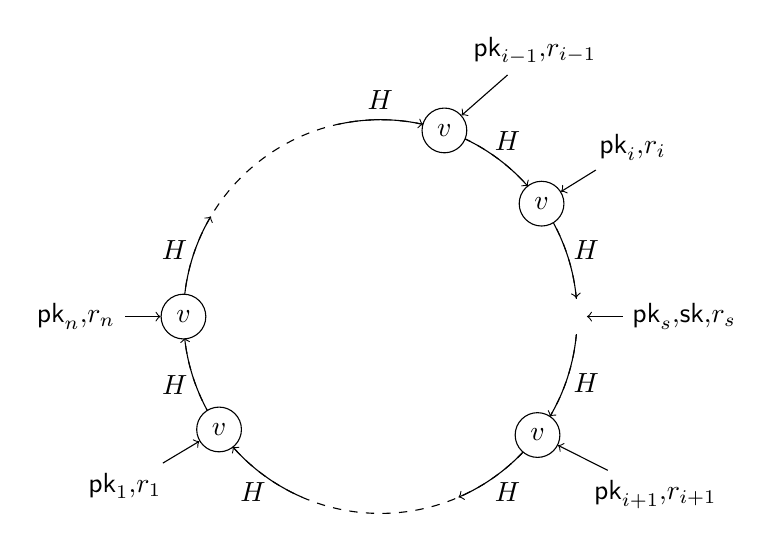
\begin{tikzpicture}[every pin edge/.style={<-}]
    \node [draw,dashed,circle through=(0:2.5)] (c) {};
    \foreach \i/\j in {0.15/0.85,1.15/1.85,2.15/2.85,4.15/4.85,5.17/5.85,6.15/6.85,8.15/8.85,9.15/9.85}
        \draw [<-] (\i/10*360:2.5) arc[radius=2.5,start angle={\i/10*360},end angle={\j/10*360}] node at ({(\i+\j)/10*360/2}:2.75) {$H$};
    \foreach \i/\j in {1/i,2/i-1,5/n,6/1,9/i+1}
        \node [draw,circle,fill=white,pin={{\i/10*360}:$\mathsf{pk}_{\j}$,$r_{\j}$}] at (c.{\i/10*360}) {$v$};
    \node [minimum height=4.5mm,fill=white,pin={0:$\mathsf{pk}_s$,$\mathsf{sk}$,$r_s$}] at (c.{10/10*360}) {};
\end{tikzpicture}

\end{document}